\documentclass[10pt]{article}
\usepackage{geometry}
\geometry{a4paper}
\usepackage[parfill]{parskip}
\usepackage[colorlinks=true,linkcolor=blue]{hyperref}
\usepackage[pdftex]{graphicx}

\hyphenpenalty=1000

\title{\textbf{CyaSSL in Webthings}}
\author{}
\date{}

\begin{document}

\maketitle
%\tableofcontents

\section{Introduction}

The IoT (Internet of Things) is a field which is deemed to expand exponentially in the near future, as more and more devices are embedded into the continuously evolving technology surrounding us. It can find an infinite number of applications, ranging from domotics to medical, automotive and agricultural industries, only to mention a few. The large-scale deployment of such systems has direct implications on integrity and confidentiality of information, issues which need to be faced carefully. That's where a lightweight embedded library such as CyaSSL is necessary.

The wider scope of \href{http://github.com/koanlogic/webthings}{Webthings} is to provide a means of closening WSNs (Wireless Sensor Networks) to the Web by bridging these very different worlds, and to provide an open framework for their deployment, all the way from motes to frontend monitoring and control applications.

Figure \ref{fig:arch} illustrates the system's high-level architecture. KINK is the core logical bridging module, which may reside on a standalone device or can be integrated into Customer Premise Equipment. Its function is to allow communication between HTTP, the most common Application Layer protocol of the Internet, and CoAP, a similar RESTful transfer protocol which has been designed by the IETF to be applied to particularly constrained scenarios such as typical WSNs. 
The diagram shows some more specific examples, such as an Energy provider gathering information from Smart Meters in a home network via the Internet $[2]$, or intelligent nodes communicating independently in a Machine to Machine configuration $[4]$.

\begin{figure}
  \centering
  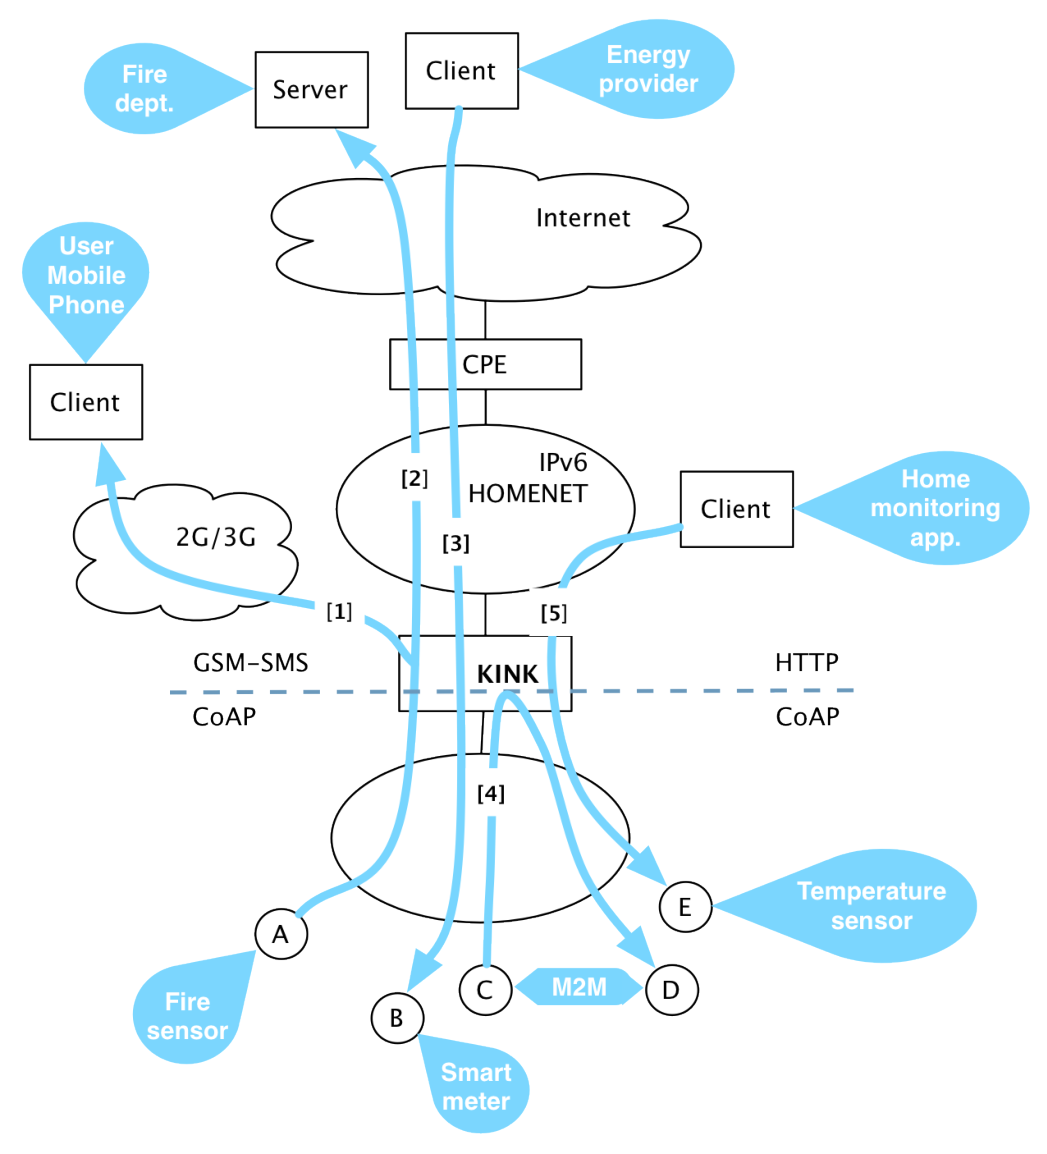
\includegraphics[width=12cm,height=12cm]{../share/images/kink-homenet}
    \caption{Webthings architecture}
    \label{fig:arch}
\end{figure}

Compared to other available solutions which are only proprietary, the advantages of applying open standards and open source to such framework should be self-evident: they promote and allow for unprecedented levels of interoperability with other systems, and extensibility of pre-existing ones. These are both key factors when such wide-usage systems are expected to constantly evolve in the direction of increasingly smart and useful solutions.

\section{Secure Communication Requirements}

Please refer to \href{http://tools.ietf.org/html/draft-ietf-core-coap-08#section-10.1}{``Securing CoAP with DTLS''} section of the CoAP I-D for a detailed overview of rationale and requirements.  Briefly, the needed items are:

\begin{itemize}
\item DTLS (\href{http://tools.ietf.org/html/rfc4347}{RFC 4347} and \href{http://tools.ietf.org/html/rfc6347}{RFC 6347});
\item Pre-Shared Key (\href{http://tools.ietf.org/html/rfc4279}{RFC 4279}) with \texttt{TLS\_PSK\_WITH\_AES\_128\_CCM\_8} cipher suite (\href{http://tools.ietf.org/html/draft-mcgrew-tls-aes-ccm-ecc-02}{I-D.mcgrew-tls-aes-ccm});
\item Raw Public Key (\href{http://tools.ietf.org/html/draft-wouters-tls-oob-pubkey}{I-D.wouters-tls-oob-pubkey}) with \texttt{TLS\_ECDHE\_ECDSA\_WITH\_AES\_128\_CCM\_8} cipher suite (\href{http://tools.ietf.org/html/rfc4492}{RFC 4492} and \href{http://tools.ietf.org/html/rfc5246}{RFC 5246});
\item Server Name Indication (\href{http://tools.ietf.org/html/rfc6066}{RFC 6066}).
\end{itemize}

\subsection{OS-level Requirements}
\label{sec:reqs-os}
Target operating systems:
\begin{enumerate}
\item\label{linux} Linux -- KINK runs a CoAP proxy on an unconstrained (yet still embedded) platform -- since this is a major target for CyaSSL no particular porting operations should be required;
\item\label{contiki} \href{http://www.contiki-os.org}{Contiki OS} -- currently working on HEAD, basic CoAP communication in place;
\item\label{tinyos} \href{http://www.tinyos.net}{TinyOS} -- currently working on HEAD, CoAP not verified yet but seems \href{http://zolertia.sourceforge.net/wiki/index.php/Blip_v2.0}{possible}.
\end{enumerate}

Should support \ref{linux} for KINK, \ref{contiki}, the main target OS for Webthings WSNs, but possibly also \ref{tinyos}.

\subsection{Constrained Target Requirements}
Target motes:
\begin{enumerate}
\item\label{z1} \href{http://www.zolertia.com/ti}{Zolertia Z1};
\item\label{tmote} \href{http://www.ti.com/tool/msp430-3p-motei-tmotesky-dsgkt}{TMote Sky/TelosB}.
\item ...
\end{enumerate}

\ref{z1} is the only target currently supported in Webthings, but the CyaSSL extension shall be hardware-independent, so many other mote types should be supported without extra effort (e.g. \ref{tmote}) -- the only limitations are given by RAM and flash sizes.

\textbf{Z1 note}: during our CoAP experiments in the constrained environments we faced some trouble due to RAM restrictions (Z1 has 8KB as shown in Appendix \ref{sec:z1-feats}). Already to run plain CoAP, some trimming is necessary to fit within these scrict limits, which should give an idea of how compact the DTLS stack needs to be in order to coexist with other layers. Some extra trimming should be possible on the networking side, for example by lightening the routing protocol or at worst by using static routes, but the remaining amount of memory available might still be less than 1KB. As far as flash ROM is concerned, the remaining memory availability for DTLS should be in the order of 20-30KB.

\section{Partnerships}
Webthings will be licensed under a very liberal open source license, most likely BSD, hence maximising the possible number of end users (from hobbyists to enterprises wanting to deploy large-scale WSNs). Given the positive predictions for this market, we believe it could be strategic for Sawtooth Consulting to contribute, sponsor and/or invest in porting its own products to the Webthings project to increase revenues given by sales of CyaSSL licenses. KoanLogic partners have already financed a substantial number of man months in the project and have applied for fundings from a EU project and NLNET, both of which are yet to be confirmed. Besides direct funding, we are also looking for new partners in order to expand the shareholders' ecosystem.

\section{Appendix}

\subsection{Zolertia Z1 Features}
\label{sec:z1-feats}
\begin{itemize}
  \item \textbf{microcontroller:} Texas Instruments MSP430F2617, 16 MHz frequency;
  \item \textbf{radio:} Chipcon CC2420 2.4 GHz IEEE 802.15.4 Wireless Transceiver;
  \item \textbf{program + data mem:} 8 KB RAM;
  \item \textbf{external memory:} 92 KB Flash;
  \item \textbf{programming:} C, nesC;
  \item \textbf{notes:} Contiki and TinyOS Support. 16 Mbit external flash + 2 digital on-board sensors (accelerometer, temperature).
\end{itemize}

\subsection{Contiki OS}
Contiki is an open source, highly portable, multi-tasking operating system for memory-efficient networked embedded systems and WSN.  The core of Contiki contains several components including uIP and Sicslopan communication stacks. uIP is a small RFC-compliant TCP/IP stack that makes it possible for Contiki to communicate over the Internet, while the Sicslopan stack realizes 6LoWPAN process according to [RFC4944] and ietf-draft-6lowpan-hc-01.  Contiki is implemented in a layered structure.  The hardware platform difference is also considered by implementing drivers for different platforms.  

\subsection{TinyOS}
The most extensive implementation of 6LoWPAN for TinyOS is called blip and it is developed at the University of California, Berkeley.  IPv6 neighbor discovery, default route selection and point-to-point routing are the most important features it supports. In addition to the IPv6 functionalities, it supports ICMP, UDP and includes a prototype TCP stack.  Although it implements lots of functionality, it still contains several known issues.  The fragmentation of IP packets used in blip can be problematic, in particular when using multi-hop.  Buffering is a second known issue: several message buffers and windows are used, consuming large amounts of memory, and causing messages to be dropped if space is exhausted. Also, the stack does not include standard IEEE 802.15.4 interfaces.  
\end{document}
